% 1st cousins and co-cousins: G is a 1st cousin of both F and H; F and H are co-cousins
% (F's uncle married H's aunt: no common ancestor, but a shared cousin, G).
\documentclass[tikz, border=4mm]{standalone}
% Shared style for the pedigree components (\input by components/pedigree_*.tex).
\usepackage[T1]{fontenc}
\usepackage{lmodern}
\usepackage[default]{sourcesans}
\usetikzlibrary{positioning, calc}

% one palette for every relationship type (Okabe-Ito, colour-blind safe)
\definecolor{cFull}{HTML}{0072B2}   % full siblings
\definecolor{cHalf}{HTML}{009E73}   % half-siblings
\definecolor{cStep}{HTML}{D55E00}   % step-siblings
\definecolor{cAdopt}{HTML}{56B4E9}  % adoptive siblings
\definecolor{cCous}{HTML}{CC79A7}   % 1st cousins
\definecolor{cCoc}{HTML}{E69F00}    % co-cousins
\definecolor{ink}{HTML}{1F2328}
\definecolor{leaf}{HTML}{DDE3EA}

\tikzset{
  ped/.style={draw=ink, line width=1.2pt},
  male/.style={ped, rectangle, minimum size=7.5mm, inner sep=0pt, fill=#1, font=\small\bfseries},
  female/.style={ped, circle, minimum size=8.2mm, inner sep=0pt, fill=#1, font=\small\bfseries},
  male/.default=white, female/.default=white,
  line/.style={ped},
  adopted/.style={ped, dash pattern=on 4pt off 3pt},
  rel/.style={line width=3.2pt, rounded corners=6pt, line cap=round},
  rellab/.style={font=\small\bfseries, fill=white, inner sep=1.5pt},
}
% connector from x1 to x2 at depth d below the leaf row (y = base), label in the middle
% \connect{colour}{x1}{x2}{depth}{label}{label position: on | below}
\newcommand{\connect}[6]{%
  \draw[rel, #1] (#2,\base) -- (#2,\base-#4) -- (#3,\base-#4) -- (#3,\base);
  \ifx#6b\node[rellab, text=#1, below=1mm] at ($(#2,\base-#4)!0.5!(#3,\base-#4)$) {#5};%
  \else\node[rellab, text=#1] at ($(#2,\base-#4)!0.5!(#3,\base-#4)$) {#5};\fi}

\begin{document}
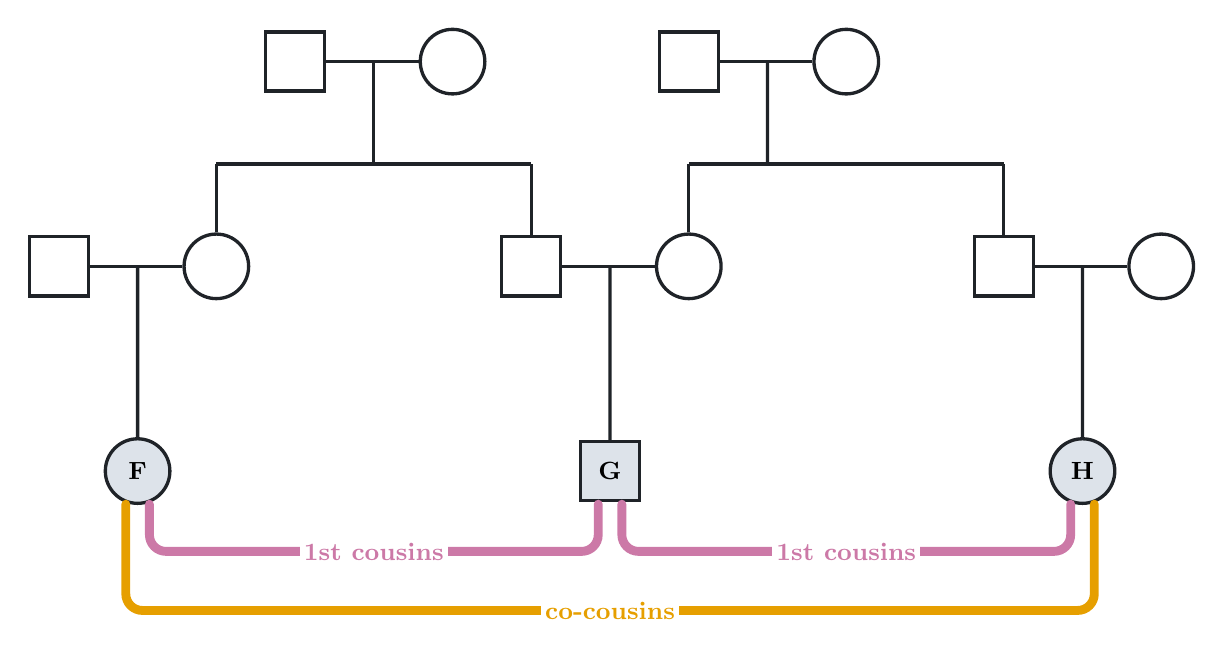
\begin{tikzpicture}[x=1cm, y=1cm]
\def\gA{0}\def\gB{-2.6}\def\gC{-5.2}\def\base{\gC-0.42}
% grandparents of two unrelated families
\node[male]   (g1m) at (4,\gA) {};  \node[female] (g1f) at (6,\gA) {};
\node[male]   (g2m) at (9,\gA) {};  \node[female] (g2f) at (11,\gA) {};
\draw[line] (g1m) -- (g1f);  \draw[line] (g2m) -- (g2f);
% parents: sibling pairs in each family; the families joined by one marriage
\node[male]   (o1) at (1,\gB)  {};   % in-law
\node[female] (s1) at (3,\gB)  {};   % family 1, daughter
\node[male]   (s2) at (7,\gB)  {};   % family 1, son
\node[female] (t1) at (9,\gB)  {};   % family 2, daughter
\node[male]   (t2) at (13,\gB) {};   % family 2, son
\node[female] (o2) at (15,\gB) {};   % in-law
\draw[line] ($(g1m)!0.5!(g1f)$) -- (5,\gB+1.3);  \draw[line] (3,\gB+1.3) -- (7,\gB+1.3);
\draw[line] (s1.north) -- (3,\gB+1.3);  \draw[line] (s2.north) -- (7,\gB+1.3);
\draw[line] ($(g2m)!0.5!(g2f)$) -- (10,\gB+1.3);  \draw[line] (9,\gB+1.3) -- (13,\gB+1.3);
\draw[line] (t1.north) -- (9,\gB+1.3);  \draw[line] (t2.north) -- (13,\gB+1.3);
\draw[line] (o1) -- (s1);  \draw[line] (s2) -- (t1);  \draw[line] (t2) -- (o2);
% leaves
\node[female=leaf] (f) at (2,\gC)  {F};
\node[male=leaf]   (g) at (8,\gC)  {G};
\node[female=leaf] (h) at (14,\gC) {H};
\draw[line] ($(o1)!0.5!(s1)$) -- (f.north);
\draw[line] ($(s2)!0.5!(t1)$) -- (g.north);
\draw[line] ($(t2)!0.5!(o2)$) -- (h.north);
% relationships
\connect{cCous}{7.85}{2.15}{0.6}{1st cousins}{o}
\connect{cCous}{8.15}{13.85}{0.6}{1st cousins}{o}
\connect{cCoc}{1.85}{14.15}{1.35}{co-cousins}{o}
\end{tikzpicture}
\end{document}
